\chapter{Modos deslizantes y super-twisting}

\begin{enpocas}
Qué es una superficie deslizante, por qué el control por modos deslizantes resiste perturbaciones
que no conoce, qué es el \emph{chattering}, cómo lo resuelve el super-twisting y por qué conviene que
su ganancia se adapte sola.
\end{enpocas}

\section{El problema: perturbaciones que no conocemos}

El PID funciona bien, pero sus ganancias se ajustan para un caso. Si el viento cambia mucho, o el dron
lleva una carga distinta, rinde peor. El \textbf{control por modos deslizantes} (SMC, \emph{sliding
mode control}) nace con otra idea: no importa cuál sea la perturbación, siempre que no pase de cierto
tamaño, el controlador la vence.

\section{La superficie deslizante}

Se define una variable que combina el error y su velocidad:
\begin{equation}
s = \dot e + \lambda e ,\qquad \lambda > 0 .
\end{equation}
Si logramos que $s = 0$, entonces $\dot e = -\lambda e$: el error decae exponencialmente a cero solo,
como $e(t) = e_0\,e^{-\lambda t}$. La recta $s = 0$ en el plano (error, velocidad del error) es la
\textbf{superficie deslizante}. El trabajo se divide en dos:
\begin{enumerate}
  \item \textbf{llegar} a la superficie, aunque haya perturbación;
  \item \textbf{quedarse} en ella y ``deslizarse'' hasta el origen.
\end{enumerate}

\begin{figure}[H]
\centering
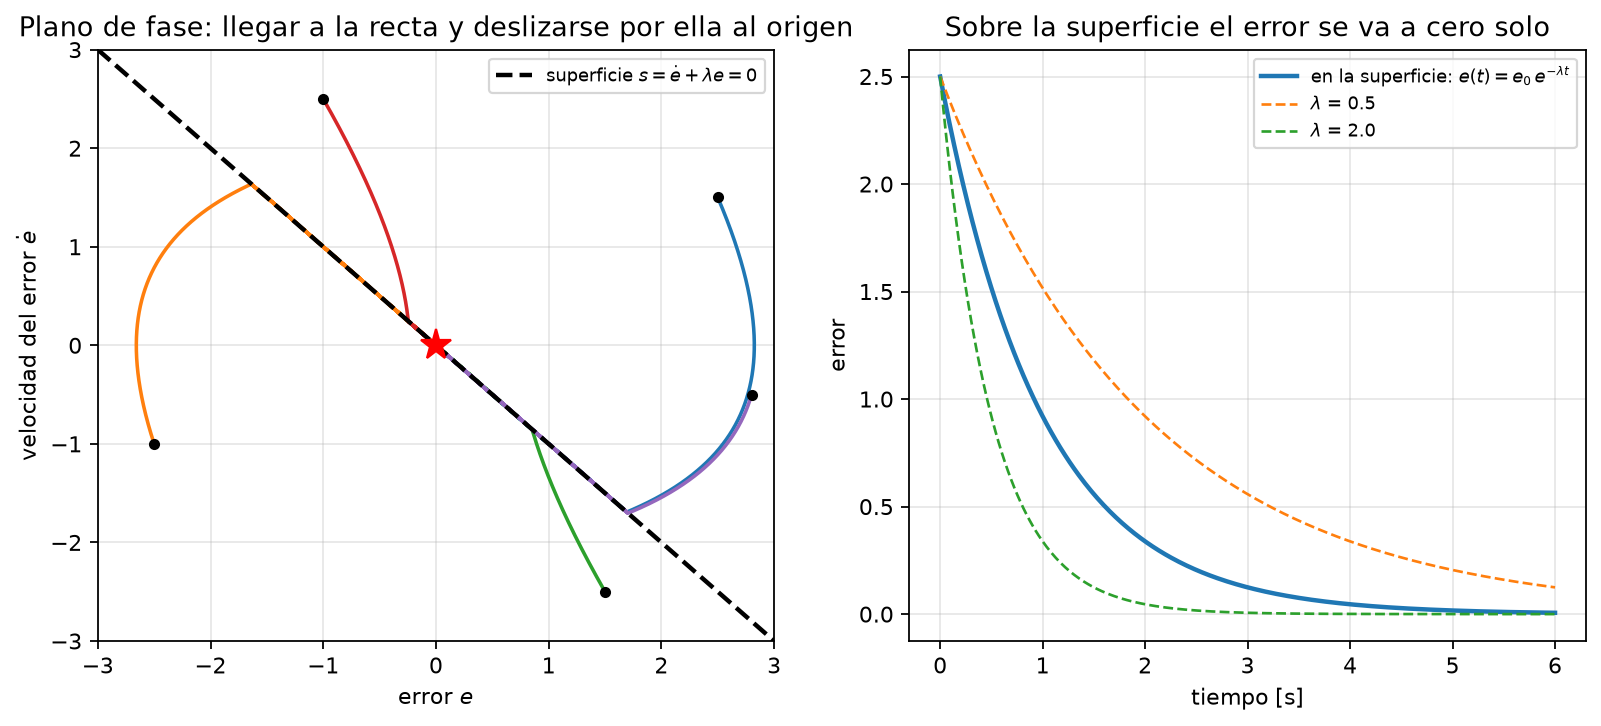
\includegraphics[width=\textwidth]{c_deslizante.png}
\caption{Izquierda: desde cualquier punto, el estado viaja hasta la recta $s=0$ y luego se desliza
por ella hasta el origen (error cero). Derecha: sobre la superficie, $\lambda$ decide qué tan rápido
se va el error.}
\label{fig:deslizante}
\end{figure}

\begin{ejemplo}
Imagina una canica en un tobogán con forma de ``V''. Caiga donde caiga, rueda hasta el fondo de la
``V'' (llegar a la superficie) y luego baja por el fondo del canal hasta la meta (deslizarse). El
viento puede empujarla, pero si las paredes son lo bastante empinadas, no la saca del canal.
\end{ejemplo}

\section{El control clásico: empujar con todo}

El SMC más simple empuja siempre con la misma fuerza hacia la superficie:
\begin{equation}
u = -k\,\sgn(s) ,
\end{equation}
donde $\sgn(s)$ vale $+1$ si $s>0$ y $-1$ si $s<0$. Si $k$ es mayor que la perturbación más grande,
el estado siempre llega a la superficie. Es muy robusto, pero tiene un problema grave.

\section{El chattering}

Al llegar a $s=0$, el control salta de $+k$ a $-k$ una y otra vez, muy rápido. Eso es el
\textbf{chattering} (``castañeteo''): vibraciones que desgastan los motores, gastan batería y pueden
excitar dinámicas que el modelo no considera.

\begin{figure}[H]
\centering
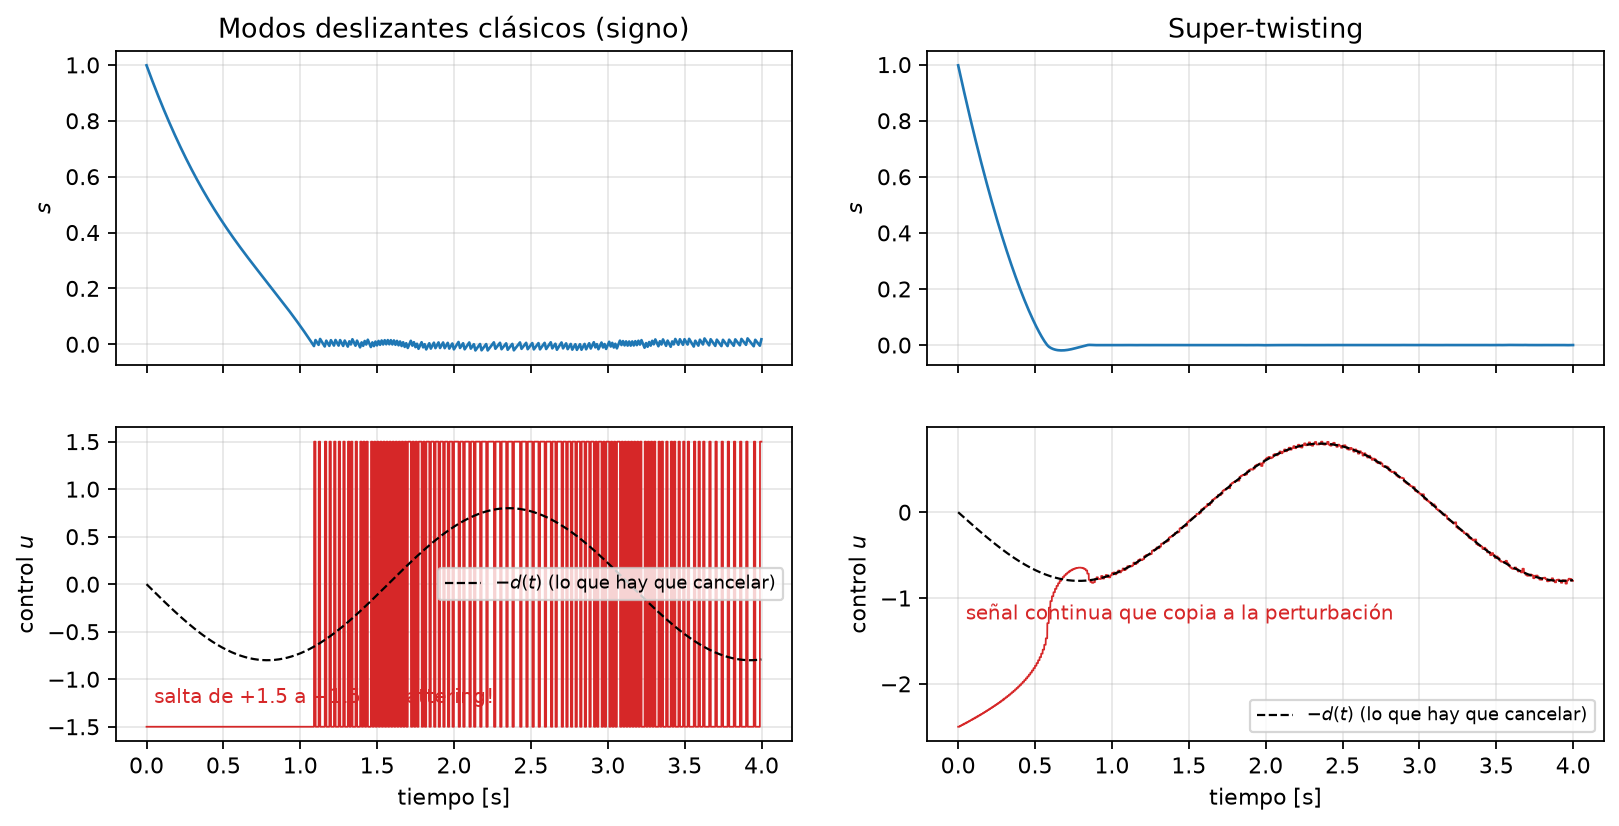
\includegraphics[width=\textwidth]{c_chattering.png}
\caption{Izquierda: el SMC clásico lleva $s$ a cero, pero su control salta sin parar entre $+1.5$ y
$-1.5$. Derecha: el super-twisting también lleva $s$ a cero, con una señal de control suave que copia
a la perturbación para cancelarla.}
\label{fig:chattering}
\end{figure}

\section{Super-twisting: robusto y suave}

El algoritmo \textbf{super-twisting} (STA) es un modo deslizante ``de segundo orden'' que esconde la
parte discontinua detrás de una integral:
\begin{align}
u &= -k_1 |s|^{1/2}\sgn(s) + \nu,\\
\dot\nu &= -k_2\,\sgn(s).
\end{align}
\begin{itemize}
  \item El primer término empuja hacia la superficie con una fuerza que se hace pequeña cerca de ella
        (por la raíz cuadrada).
  \item El segundo, $\nu$, es la integral de un signo: va creciendo o decreciendo poco a poco hasta
        igualar a la perturbación. Como una integral es continua, \textbf{el control $u$ es continuo}.
\end{itemize}
El resultado: $s$ y $\dot s$ llegan a cero en tiempo finito, aunque haya una perturbación que cambie
(con derivada acotada), y sin chattering en el control continuo (figura~\ref{fig:chattering},
derecha).

\begin{recuerda}
El super-twisting tiene la robustez de los modos deslizantes pero entrega una señal de control
continua. Necesita dos ganancias, $k_1$ y $k_2$, lo bastante grandes para la perturbación.
\end{recuerda}

\section{Ganancia adaptativa: no exagerar}

¿Qué tan grandes deben ser $k_1$ y $k_2$? Si son pequeñas, una ráfaga fuerte gana; si son grandes,
el control es agresivo todo el tiempo y amplifica el ruido. La versión \textbf{adaptativa} (Shtessel,
Taleb y Plestan, 2012) las ajusta sola:
\begin{equation}
\dot k_1 = \begin{cases} +w_1\sqrt{\gamma_1/2} & \text{si } |s| > \mu \ \text{(vamos mal: subir)}\\
                          -w_1\sqrt{\gamma_1/2} & \text{si } |s| < \mu \ \text{(vamos bien: bajar)}\end{cases}
\qquad k_2 = 2\varepsilon k_1 .
\end{equation}
$\mu$ es una pequeña tolerancia: si $s$ se mantiene dentro de $\pm\mu$, la ganancia baja; si se sale,
sube.

\begin{figure}[H]
\centering
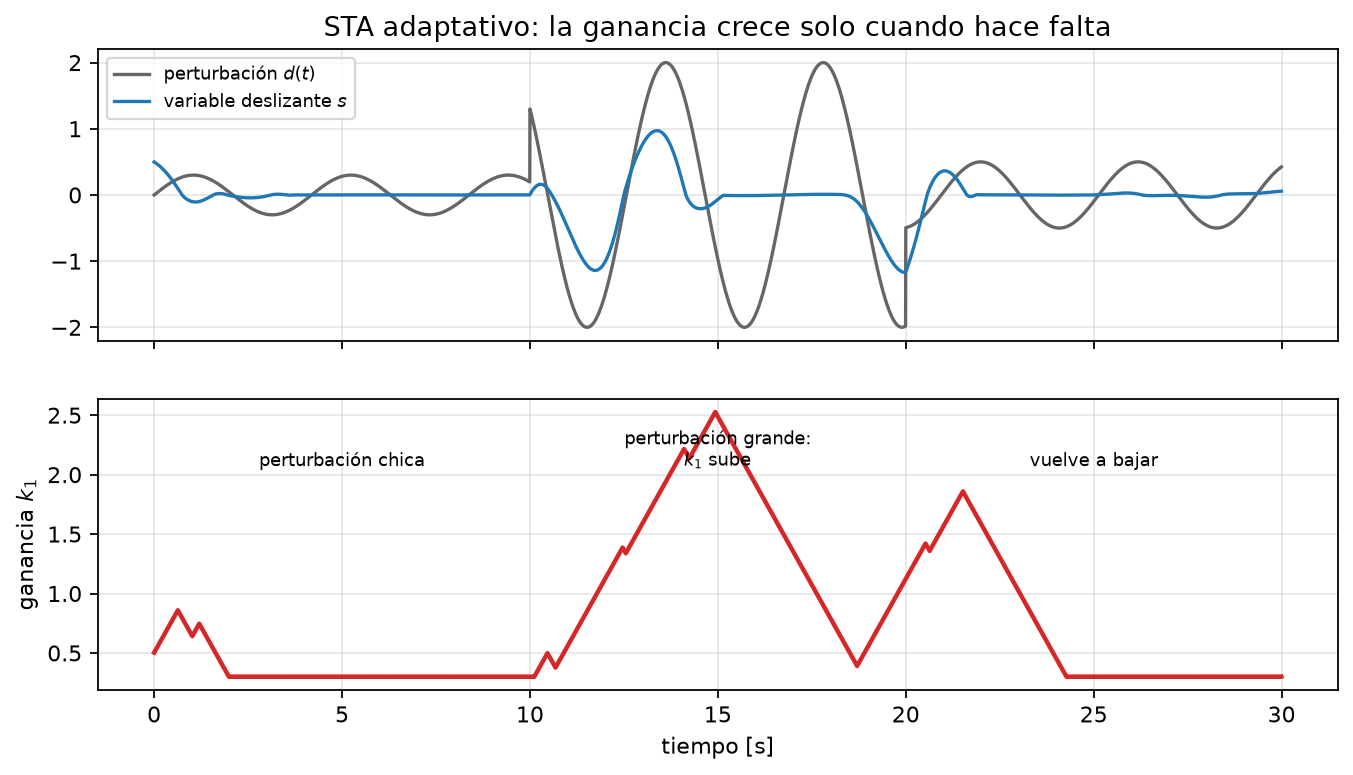
\includegraphics[width=0.85\textwidth]{c_adaptativo.png}
\caption{La perturbación crece de $t=10$ a 20~s: la ganancia $k_1$ sube para vencerla y luego vuelve a
bajar.}
\end{figure}

\begin{aviso}
Elegir $\mu$ es delicado. En el dron, el retardo de los motores y del lazo de actitud produce una
pequeña oscilación de $s$ que nunca desaparece (un \emph{ciclo límite}). Si $\mu$ es menor que esa
oscilación, la ganancia crece sin parar y el dron se vuelve inestable. Por eso en la simulación $\mu$
es distinto para cada eje y cada vehículo (0.3~m/s en $x$, $y$ y 0.03~m/s en $z$ para el Tarot).
\end{aviso}

\section{Cómo se usa en el dron}

Por cada eje ($x$, $y$, $z$) del lazo de posición:
\begin{equation}
s = e_v + \lambda e_p ,\qquad a = a_d + \lambda e_v - u ,
\end{equation}
donde $e_p$ y $e_v$ son los errores de posición y velocidad y $a_d$ la aceleración que pide la
trayectoria. Con esa elección resulta $\dot s = u + d$: exactamente el sistema para el que está
diseñado el super-twisting, con $d$ la perturbación (viento y todo lo que el modelo no sabe). Los
detalles están en el capítulo~\ref{cap:control-sim}.
